\documentclass[10pt,A4]{article}
\usepackage[utf8]{inputenc}
\usepackage{xifthen}
\usepackage[default]{gillius}
\renewcommand*\familydefault{\sfdefault}
\usepackage[T1]{fontenc}
\usepackage{moresize}
\usepackage{fontawesome}
\usepackage[a4paper]{geometry}
\geometry{top=1cm, bottom=-.6cm, left=0.4cm, right=1cm}
\setlength{\headheight}{-5pt}
\setlength{\parindent}{0mm}
\usepackage{multicol}
\usepackage{multirow}
\usepackage{array}
\newcolumntype{x}[1]{%
>{\raggedleft\hspace{0pt}}p{#1}}%
\usepackage{graphicx}
\usepackage{wrapfig}
\usepackage{float}
\usepackage{tikz}
\usetikzlibrary{shapes, backgrounds,mindmap, trees}
\usepackage{transparent}
\usepackage{color}

% main colors
\definecolor{complcol}{RGB}{244,160,0}
\definecolor{bgcol}{RGB}{110,110,110}
\definecolor{softcol}{RGB}{219,68,55}
\definecolor{sectcol}{RGB}{66,133,244}
\definecolor{maya}{RGB}{124,185,232}
% pie chart colors
\definecolor{col1}{RGB}{66,133,244}
\definecolor{col2}{RGB}{219,68,55}
\definecolor{col3}{RGB}{244,160,0}
\definecolor{col4}{RGB}{15,157,88}
\definecolor{col5}{RGB}{251, 120, 56}

\usepackage[hidelinks]{hyperref}

\newcommand{\mpwidth}{\linewidth-\fboxsep-\fboxsep}

\newcommand{\tzlarrow}{(0,0) -- (0.2,0) -- (0.3,0.2) -- (0.2,0.4) -- (0,0.4) -- (0.1,0.2) -- cycle;}

% include the left arrow into a tikz picture
% param1: fill color
%
\newcommand{\larrow}[1]
{\begin{tikzpicture}[scale=0.58]
	 \filldraw[fill=#1!100,draw=#1!100!black]  \tzlarrow
 \end{tikzpicture}
}

% a six pointed arrow poiting to the right
\newcommand{\tzrarrow}{ (0,0.2) -- (0.1,0) -- (0.3,0) -- (0.2,0.2) -- (0.3,0.4) -- (0.1,0.4) -- cycle;}

% include the right arrow into a tikz picture
% param1: fill color
%
\newcommand{\rarrow}
{
\begin{tikzpicture}[scale=0.7]
	\filldraw[fill=softcol!100,draw=softcol!100!black] \tzrarrow
 \end{tikzpicture}
}

%----------------------------------------------------------------------------------------
%	custom sections
%----------------------------------------------------------------------------------------

% create a coloured box with arrow and title as cv section headline
% param 1: section title
%
\newcommand{\cvsection}[1]
{
\colorbox{sectcol}{\mystrut \makebox[1\mpwidth][l]{
\larrow{softcol} \hspace{-8pt} \larrow{softcol} \hspace{-8pt} \larrow{softcol} \textbf{\textcolor{white}{\uppercase{#1}}}\hspace{4pt}
}}\\
}

\newcommand{\cvskill}[3] {
	\begin{tabular*}{1\mpwidth}{p{0.75\mpwidth}  r}
		\textcolor{white}{\textbf{#1}} & \textcolor{white}{\textbf{#2}}\\
	\end{tabular*}%
	\hspace{1pt}
	\begin{tikzpicture}[scale=1,rounded corners=2pt,very thin]
	\fill [white] (0,0) rectangle (1\mpwidth, 0.15);
	\fill [col4] (0,0) rectangle (#3\mpwidth, 0.15);
	\end{tikzpicture}%
}

% create a coloured arrow with title as cv meta section section
% param 1: meta section title
%
\newenvironment{metasection}[1] {
	\vspace{6pt}
	\begin{center}
		\textcolor{white}{\large{\uppercase{#1}}}\\
	\normalsize
	\parbox{0.7\mpwidth}{\textcolor{white}	\hrule}
}{\end{center}}

%----------------------------------------------------------------------------------------
%	 CV EVENT
%----------------------------------------------------------------------------------------

% creates a stretched box as cv entry headline followed by two paragraphs about
% the work you did
% param 1:	event time i.e. 2014 or 2011-2014 etc.
% param 2:	event name (what did you do?)
% param 3:	institution (where did you work / study)
% param 4:	what was your position
% param 5:	some words about your contributions
%
\newcommand{\cvevent}[5]
{
\vspace{8pt}
	\begin{tabular*}{1\mpwidth}{p{0.55\mpwidth}  x{0.42\mpwidth}}
 	\textcolor{black}{\textbf{#2}} & \textcolor{softcol}{#3}, \textcolor{bgcol}{\textbf{#1}}

	\end{tabular*}
\vspace{-12pt}
\textcolor{softcol}{\hrule}
\vspace{6pt}
	\begin{tabular*}{0.5\mpwidth}{p{\mpwidth}}
\larrow{softcol}  #4\\[3pt]
\larrow{softcol}  #5\\[6pt]
	\end{tabular*}

}

% creates a stretched box as
\newcommand{\cveventmeta}[2]
{
	\mbox{\mystrut \hspace{87pt}\textit{#1}}\\
	#2
}

%----------------------------------------------------------------------------------------
% CUSTOM STRUT FOR EMPTY BOXES
%----------------------------------------- -----------------------------------------------
\newcommand{\mystrut}{\rule[-.3\baselineskip]{0pt}{\baselineskip}}

%----------------------------------------------------------------------------------------
% CUSTOM LOREM IPSUM
%----------------------------------------------------------------------------------------
\newcommand{\lorem}
{Lorem ipsum dolor sit amet, consectetur adipiscing elit. Donec a diam lectus.}


% use to vertically center content
% credits to: http://tex.stackexchange.com/questions/7219/how-to-vertically-center-two-images-next-to-each-other
\newcommand{\vcenteredinclude}[1]{\begingroup
\setbox0=\hbox{\includegraphics{#1}}%
\parbox{\wd0}{\box0}\endgroup}

% use to vertically center content
% credits to: http://tex.stackexchange.com/questions/7219/how-to-vertically-center-two-images-next-to-each-other
\newcommand*{\vcenteredhbox}[1]{\begingroup
\setbox0=\hbox{#1}\parbox{\wd0}{\box0}\endgroup}

%----------------------------------------------------------------------------------------
%	ICON-SET EMBEDDING
%----------------------------------------------------------------------------------------

% at this point we simplify our icon-embedding by simply referring to a set of png images.
% if you find a good way of including svg without conflicting with other packages you can
% replace this part
\newcommand{\icon}[3]{\makebox(#2, #2){\textcolor{#3}{\csname fa#1\endcsname}}}	%icon shortcut
\newcommand{\icontext}[4]{ 						%icon with text shortcut
	\vcenteredhbox{\icon{#1}{#2}{#4}} \vcenteredhbox{\textcolor{#4}{#3}}
}
\newcommand{\iconhref}[5]{ 						%icon with website url
    \vcenteredhbox{\icon{#1}{#2}{#5}} \href{#4}{\textcolor{#5}{#3}}
}

\newcommand{\iconemail}[5]{ 						%icon with email link
    \vcenteredhbox{\icon{#1}{#2}{#5}} \href{mailto:#4}{\textcolor{#5}{#3}}
}

%----------------------------------------------------------------------------------------
% 	PIE CHART
%----------------------------------------------------------------------------------------
%-----------------------------------------------------------------------------------------------------------------------------------------------%
%	The MIT License (MIT)
%
%	Copyright (c) 2016 Jan Küster
%
%	Permission is hereby granted, free of charge, to any person obtaining a copy
%	of this software and associated documentation files (the "Software"), to deal
%	in the Software without restriction, including without limitation the rights
%	to use, copy, modify, merge, publish, distribute, sublicense, and/or sell
%	copies of the Software, and to permit persons to whom the Software is
%	furnished to do so, subject to the following conditions:
%	
%	THE SOFTWARE IS PROVIDED "AS IS", WITHOUT WARRANTY OF ANY KIND, EXPRESS OR
%	IMPLIED, INCLUDING BUT NOT LIMITED TO THE WARRANTIES OF MERCHANTABILITY,
%	FITNESS FOR A PARTICULAR PURPOSE AND NONINFRINGEMENT. IN NO EVENT SHALL THE
%	AUTHORS OR COPYRIGHT HOLDERS BE LIABLE FOR ANY CLAIM, DAMAGES OR OTHER
%	LIABILITY, WHETHER IN AN ACTION OF CONTRACT, TORT OR OTHERWISE, ARISING FROM,
%	OUT OF OR IN CONNECTION WITH THE SOFTWARE OR THE USE OR OTHER DEALINGS IN
%	THE SOFTWARE.
%
%-----------------------------------------------------------------------------------------------------------------------------------------------%

%counters for chart loop
\newcounter{a}
\newcounter{b}
\newcounter{c}

% draw a slice for a chart
% param 1: Circle form - 90 = quarter, 180 = half, 360 = full
% param 2: scale default=1 (scales only chart, not label text)
% param 3: border color
% param 4: label text color
% param 5: label bg color
% param 6:
\newenvironment{piechart}[5] {

	% draw a slice for a chart
	% param 1: value x of 100
	% param 2: label text
	% param 3: fill color
	% param 4:
	% param 5:
	% param 6:
	\newcommand{\slice}[3] {

		\setcounter{a}{\value{b}}
		\addtocounter{b}{##1}

		%set from angle point
		\pgfmathparse{\thea/100*#1}
	  	\let\pointa\pgfmathresult

		%set toanglepoint
		\pgfmathparse{\theb/100*#1}
	  	\let\pointb\pgfmathresult

		%set midangle
	 	\pgfmathparse{0.5*\pointa+0.5*\pointb}
	  	\let\midangle\pgfmathresult
		
		% draw the slice
	  	\filldraw[fill=##3!100,draw=#3!100, line width=1pt ] (0,0) -- (\pointa:#2) arc (\pointa:\pointb:#2) -- cycle;

	  	% draw label
	  	\node[label=\midangle:\hspace{10mm}\textcolor{#4}{\hspace{-9mm}##2}] at (\midangle:#2) {};
		
		%\filldraw[fill=#3,draw=none] (0,0) circle (#2/2);
	}

	% execute commands
	\setcounter{a}{0}
	\setcounter{b}{0}
	\begin{tikzpicture}
}
{\end{tikzpicture}}


\begin{document}
%============================================================================%
%	DOCUMENT CONTENT
%============================================================================%
\fcolorbox{white}{white}{\begin{minipage}[c][0.96\textheight][t]{0.7\linewidth}

%---------------------------------------------------------------------------------------
%	HEADER SECTION
%----------------------------------------------------------------------------------------

%---------------------------------------------------------------------------------------
%	TITLE HEADLINE
%----------------------------------------------------------------------------------------
\vspace{-3pt}
% use this for multiple words like working titles etc.
%\hspace{-0.25\linewidth}\colorbox{bgcol}{\makebox[1.5\linewidth][c]{\hspace{46pt}\HUGE{\textcolor{white}{\uppercase{M.Sc. Jan Küster}} } \textcolor{sectcol}{\rule[-1mm]{1mm}{0.9cm}} \parbox[b]{5cm}{   \large{ \textcolor{white}{{IT Consultant}}}\\
% \large{ \textcolor{white}{{JS Fullstack Engineer}}}}
%}}
% use this for single words, e.g. CV or RESUME etc.
\colorbox{bgcol}{\makebox[\mpwidth][c]{\HUGE{\textcolor{white}{\uppercase{Alan Matzumiya}} } }}

%----------------------------------------------------------------------------------------
%	HEADER IMAGE
%----------------------------------------------------------------------------------------

%\includegraphics[trim= 0 250 0 270,clip,width=1\linewidth+3.1cm]{myfoto.jpg}	%trimming relative to image size!
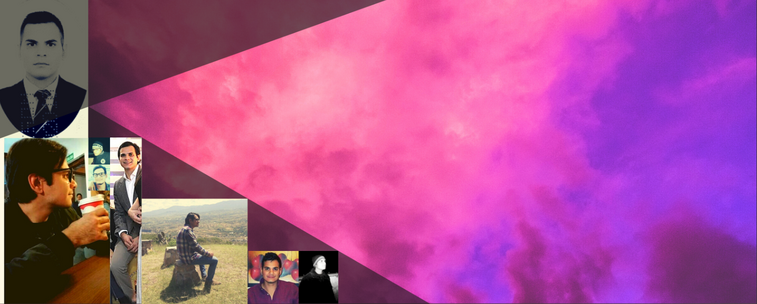
\includegraphics[width=0.9995\linewidth]{../../img/banner.png}	%trimming relative to image size

%---------------------------------------------------------------------------------------
%	SUMMARY
%----------------------------------------------------------------------------------------
\transparent{0.85}%
\vspace{-127pt}
\hspace{0.32\linewidth}
\colorbox{bgcol}{
    \parbox{0.60\linewidth}{\vspace{-1.15mm}\hspace{-2.28mm}\colorbox{softcol}{\parbox{1.028\linewidth}{\textcolor{white}{\hspace{0.22\linewidth}Alan Daniel Matzumiya Zazueta}}}
        \vspace{-4.5mm}
        \transparent{1}%
        \begin{center}
            \larrow{softcol}\larrow{softcol} \textcolor{white}{Soy Ingeniero Qu\'imico y Maestro en Ciencias Matem\'aticas. Adem\'as, Cuento con Fuertes Conocimientos en Desarrollo de Software / Web}
        \end{center}
    }
}
\vspace{59.5pt}
\transparent{1}%

%============================================================================%
%
%	MAIN CONTENT
%
%============================================================================%

%---------------------------------------------------------------------------------------
%	STATUS
%----------------------------------------------------------------------------------------
\cvsection{Acerca de Mi}

\colorbox{sectcol}{
	\parbox{0.969\linewidth}{
		\parbox{0.45\linewidth}{
			\begin{itemize}
				\item[\larrow{softcol}] \textcolor{white}{\textbf{Edad: 30 años}}
				\item[\larrow{softcol}] \textcolor{white}{\textbf{Nacimiento: 14 Sept 1992}}
				\item[\larrow{softcol}] \textcolor{white}{\textbf{Lugar de Origen: Guaymas, Son}}
				\item[\larrow{softcol}] \textcolor{white}{\textbf{Residencia: Hermosillo, Son}}				
			\end{itemize}
		}
		\parbox{0.4\linewidth}{
			\begin{itemize}
    			\item[\larrow{softcol}] \textcolor{white}{\textbf{Estado Civil: Soltero}}
				\item[\larrow{softcol}]	\cvskill{Hablar Ingl\'es} {80 \%} {0.8}
				\item[\larrow{softcol}]	\cvskill{Escribir Ingl\'es} {90 \%} {0.9}
			\end{itemize}
		}
	}
}
\vspace{5pt}

%---------------------------------------------------------------------------------------
%	EXPERIENCE
%----------------------------------------------------------------------------------------
\cvsection{Experiencia}

%
\cvevent{May-Ago 2015}{Pr\'acticas Profesionales}{CFE, Hermosillo}{Estancia de pr\'acticas profesionales que se llevo acabo en la planta: Central\\ Ciclo Combinado de Hermosillo}{El objetivo fue orientarme en la funci\'on del ingeniero qu\'imico de la central el\'ectrica,\\ la cual se desarrolla en gran parte en el proceso de tratado de agua de la planta}

%\textcolor{softcol}{\hrule}

%
\cvevent{Jun-Sep 2018}{Investigaci\'on Cient\'ifica}{UNAM, Oaxaca}{Estudio acerca de m\'etodos numericos para resolver EDP's estoc\'asticas}{Puede consultar art\'iculo publicado desde el siguiente bot\'on \hspace{10mm} \href{https://www.researchgate.net/publication/334330862_INITIAL_CONDITIONS_CONTINUITY_OF_A_NUMERICAL_APPROXIMATION_FOR_KOLMOGOROV_EQUATIONS/}{\colorbox{bgcol}{\colorbox{white}{\hspace{3mm}\textcolor{bgcol}{\textbf{Get Info}} \hspace{1.5mm} \icon{Info}{8}{bgcol}\hspace{3mm}}}}}

%\textcolor{softcol}{\hrule}

%
\cvevent{2017 - 2019}{Talleres de Programaci\'on}{Unison, Hermosillo}{Instructor en cursos de programaci\'on desarrollados en Jupyter Notebook usando\\ lenguaje Python orientados a estudiantes de ingenieria}{Puede consultar material de clase desde el siguiente bot\'on. \hspace{10mm} \href{https://github.com/CircuitalMinds/jupyter/tree/main/nbs/}{\colorbox{bgcol}{\colorbox{white}{\hspace{0.5mm}\textcolor{bgcol}{\textbf{Notebooks}} \hspace{1.5mm} \icon{Github}{8}{bgcol} \hspace{0.5mm}}}}}\textbf{Contraseña: circuitalminds}
%\textcolor{softcol}{\hrule}

%
\cvevent{2019 - Now}{Proyectos de Programaci\'on}{GitHub}{
	Paquete de Python para resolver PDE's o SPDE's construyendo\\ m\'etodos num\'ericos espectrales
	\vspace{0mm}
	}
{
	Puede consultar el proyecto desde el siguiente bot\'on: \hspace{18mm} \href{https://www.github.com/alanmatzumiya/pySpectralPDE/}{\colorbox{bgcol}{\colorbox{white}{\hspace{1mm}\textcolor{bgcol}{\textbf{Repository}} \hspace{1.5mm} \icon{Github}{8}{bgcol}\hspace{1mm}}}
	}
}

\vspace{0pt}
%---------------------------------------------------------------------------------------
%	EDUCATION SECTION
%--------------------------------------------------------------------------------------
\cvsection{Educacion}

\cvevent{2017 - 2019}{
	Grado de Maestr\'ia en Ciencias Matem\'aticas}{Unison, Hermosillo}{Tesis: Numerical Solutions to the Stochastic and Deterministic Burgers Equation Using Spectral Methods
}
{
	Click en el siguiente bot\'on para descargar archivo de tesis: \hspace{10.5mm} \href{https://raw.githubusercontent.com/alanmatzumiya/alanmatzumiya.github.io/main/assets/portfolio/master/thesis.pdf}{\colorbox{bgcol}{\colorbox{white}{\textcolor{bgcol}{\hspace{3mm}\textbf{Get PDF}} \hspace{1.5mm} \icon{Download}{8}{bgcol}\hspace{3mm}}}}
}

%\textcolor{sectcol}{\hrule}
%
\cvevent{2011 - 2016}{Licenciatura en Ingenier\'ia Qu\'imica}{Unison, Hermosillo}{
	Tesis: Caracterizaci\'on y evaluaci\'on de las propiedades bioactivas de una mezcla de biocomp\'ositos de hidroxiapatita/$\beta$-wollastonita
}
{
	Click en el siguiente bot\'on para descargar archivo de tesis: \hspace{10.5mm} \href{https://raw.githubusercontent.com/alanmatzumiya/alanmatzumiya.github.io/main/assets/portfolio/bachelor/thesis.pdf}{\colorbox{bgcol}{\colorbox{white}{\textcolor{bgcol}{\hspace{3mm}\textbf{Get PDF}} \hspace{1.5mm} \icon{Download}{8}{bgcol}\hspace{3mm}}}}
}

%---------------------------------------------------------------------------------------
%	SIDEBAR SECTION
%--------------------------------------------------------------------------------------

\end{minipage}}%
\fcolorbox{white}{sectcol}{\begin{minipage}[c][0.96\textheight][t]{0.33\linewidth}


		\begin{metasection}{Contacto}

			\icontext{MapMarker}{12}{Hermosillo, Sonora}{white}\\[6pt]

			\iconhref{Whatsapp}{12}{\textbf{+52 662 364 8525}}{https://api.whatsapp.com/send?phone=5216623648525\&text=Hola\%20Alan,\%20Buen\%20D\%C3\%ADa.}{white}\\[6pt]

			\iconemail{Send}{12}{\textbf{alan.matzumiya@gmail.com}}{alan.matzumiya@gmail.com}{white}\\[6pt]

			\iconhref{Link}{12}{\textbf{alanmatzumiya.github.io}}{https://alanmatzumiya.github.io/}{white}\\[6pt]

			\LARGE{
				\href{https://www.github.com/alanmatzumiya/}{\icon{Github}{12}{white}}
				\hspace{1mm}
				\href{https://www.linkedin.com/in/alanmatzumiya/}{\icon{LinkedinSquare}{12}{white}}
				\hspace{1mm}
				\href{https://www.facebook.com/alanmatzumiya/}{\icon{FacebookOfficial}{12}{white}}
				\hspace{1mm}
				\href{https://www.instagram.com/alanmatzumiya/}{\icon{Instagram}{12}{white}}
				\hspace{1mm}
				\href{https://www.pinterest.com/alanmatzumiya/}{\icon{Pinterest}{12}{white}}}

		\end{metasection}
		%----------------------------------------------------------------------------------------
		%	META SECTION
		%----------------------------------------------------------------------------------------

		\begin{metasection}{Aptitudes y Habilidades}

			\vspace{2pt}

			\textcolor{white}{\textbf{Liderazgo, Organizacion, Planificacion, Trabajo en equipo, Iniciativa}}
			\\

			\vspace{2pt}

			\icontext{Tasks}{12}{Desarrollo de Software / Web}{white}\\
			\icon{Star}{12}{complcol}\icon{Star}{12}{complcol}\icon{Star}{12}{complcol}\icon{Star}{12}{complcol}\icon{Star}{12}{complcol}\icon{Star}{12}{complcol}\icon{Star}{12}{complcol}\icon{Star}{12}{complcol}\icon{Star}{12}{white}\icon{Star}{12}{white}\\[6pt]

			\icontext{BarChart}{12}{Algoritmos Num\'ericos/An\'alisis de Datos}{white}\\
			\icon{Star}{12}{complcol}\icon{Star}{12}{complcol}\icon{Star}{12}{complcol}\icon{Star}{12}{complcol}\icon{Star}{12}{complcol}\icon{Star}{12}{complcol}\icon{Star}{12}{complcol}\icon{Star}{12}{complcol}\icon{Star}{12}{complcol}\icon{Star}{12}{complcol}\\[6pt]

			\cvskill{\icontext{Code}{12}{Python / JavaScript}{white}} {9+ a} {1} \\[6pt]
			\cvskill{\icontext{Code}{12}{Visual Basic / PHP}{white}} {10+ a} {0.85} \\[6pt]
			\cvskill{\icontext{Code}{12}{C++ / Fortran}{white}} {10+ a} {1} \\[6pt]
			\cvskill{\icontext{AreaChart}{12}{R / Matlab}{white}} {9+ a} {0.90} \\[6pt]
			\cvskill{\icontext{Code}{12}{HTML / CSS / Markdown}{white}} {7+ a} {0.95} \\[6pt]
			\cvskill{\icontext{Database}{12}{MySQL / MariaDB}{white}} {7+ a} {0.90}

		\end{metasection}

		\begin{metasection}{Tecnolog\'ias}

			\textcolor{white}{\LARGE{\icon{Linux}{24}{white} \icon{Windows}{24}{white}} \icon{Android}{24}{white}}\\[6pt]

			\icontext{GithubAlt}{12}{Git /}{white}  \icontext{Check}{12}{Selenium /}{white}
			\icontext{Exchange}{12}{Docker}{white} \\[6pt]

			\icontext{Server}{12}{Django / Flask / Dash}{white} \\[6pt]

			\icontext{Google}{12}{Google Analytics}{white} \icontext{Android}{12}{Android Studio}{white} \\[6pt]

			\icontext{Code}{12}{PyCharm / Visual Studio}{white}\\[6pt]

			\icontext{LineChart}{12}{Jupyter Notebook / RStudio}{white}

		\end{metasection}

		\begin{metasection}{Actividades}

		\vspace{6pt}

		\begin{piechart}{360}{-2}{maya}{maya}{white}
			\slice{40}{\LARGE{\icon{Desktop}{2}{white}}}{col2}
			\slice{30}{\LARGE{\icon{Bicycle}{8}{white}}}{col4}
			\slice{30}{\LARGE{\icon{Headphones}{0}{white}}}{col3}
		\end{piechart}

		\end{metasection}

\end{minipage}}


%-------------------------------------------------------------------------------------------------
%	ARTIFICIAL FOOTER (fancy footer cannot exceed linewidth)
%--------------------------------------------------------------------------------------------------

\null
\vspace*{\fill}
\hspace{-0.25\linewidth}\colorbox{bgcol}{
	\makebox[1.45\linewidth][c]{
		\mystrut \small \textcolor{white}{
			Coypright 2023 Alan Matzumiya}
	}
}

\vspace{1mm}
\newpage

%---------------------------------------------------------------------------------------
%	RECORDS SECTION
%--------------------------------------------------------------------------------------

%---------------------------------------------------------------------------------------
%	Records
%----------------------------------------------------------------------------------------
\colorbox{maya}{
\parbox{1.0\linewidth}{
	\colorbox{white}{
		\parbox{0.98\linewidth}{
			\cvsection{Distinciones}
			\parbox{0.5\linewidth}{
				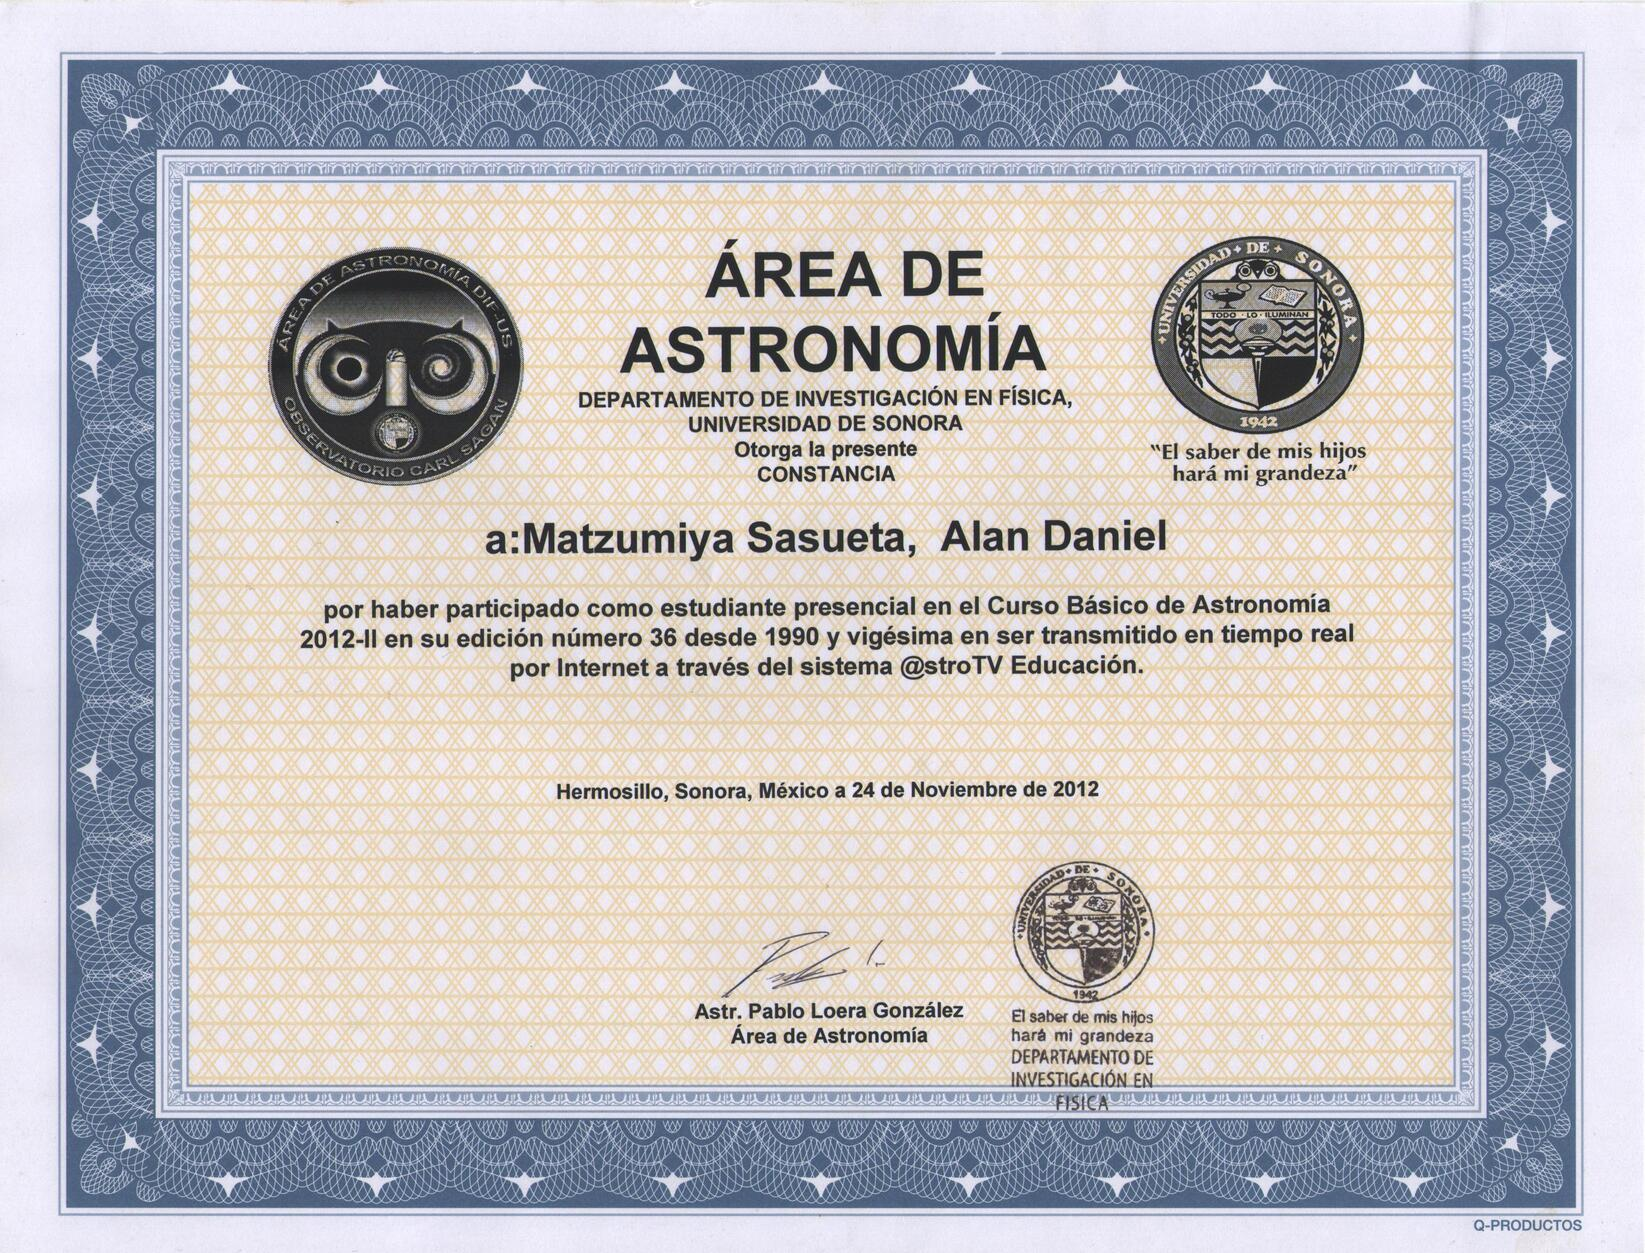
\includegraphics[width=1.0\linewidth]{../../docs/astronomy.jpeg}
				}
			\parbox{0.5\linewidth}{
				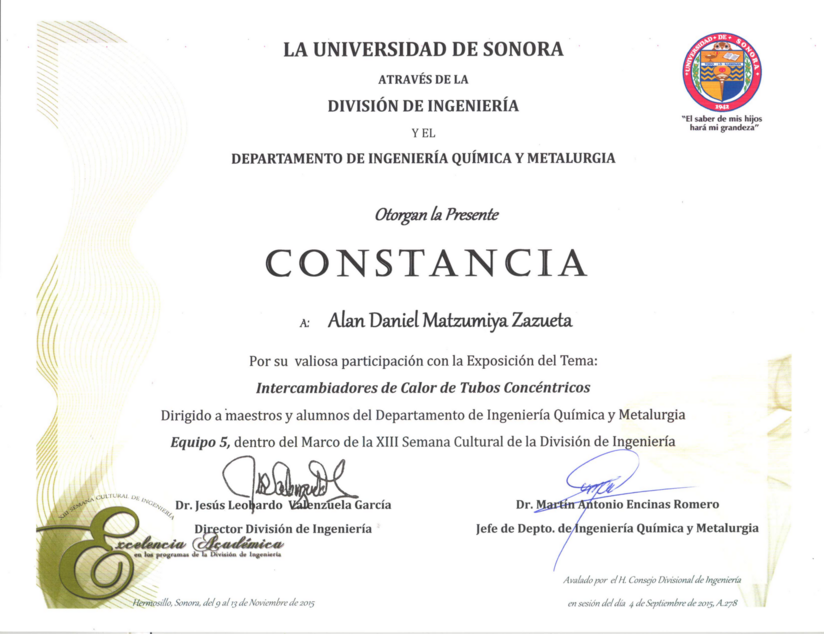
\includegraphics[width=1.0\linewidth]{../../docs/laboratory.png}
				}
			\parbox{0.5\linewidth}{
				
\includegraphics[width=1.0\linewidth]{../../docs/workshop-python-2017.pdf}
				}
			\parbox{0.5\linewidth}{
				
\includegraphics[width=1.0\linewidth]{../../docs/workshop-python-2018.pdf}
				}
			\parbox{0.5\linewidth}{
				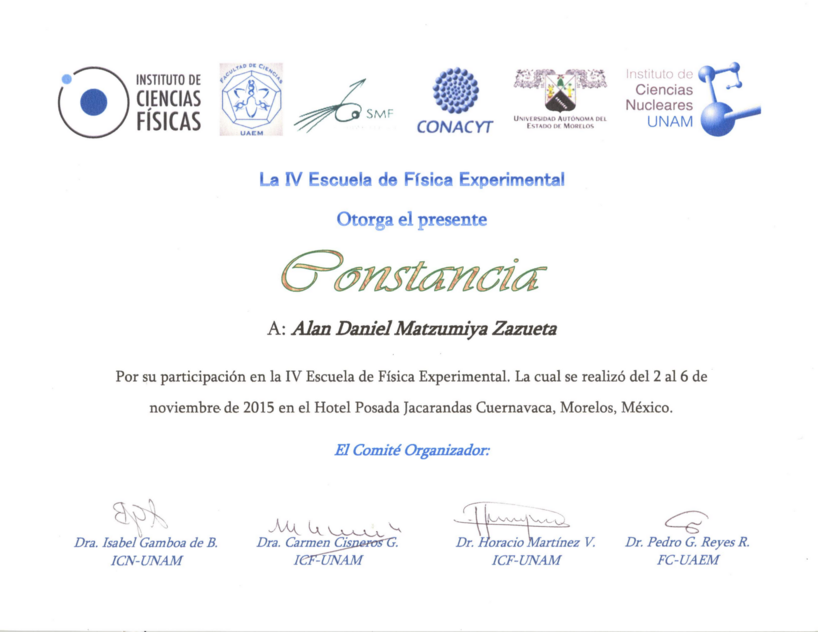
\includegraphics[width=1.0\linewidth]{../../docs/nuclear-physics.png}
				}
			}
		}
	}
}


\null
\vspace*{\fill}
\hspace{-0.25\linewidth}\colorbox{bgcol}{
	\makebox[1.45\linewidth][c]{
		\mystrut \small \textcolor{white}{
			Coypright 2023 Alan Matzumiya}
	}
}

\vspace{1mm}
\end{document}
%============================================================================%
%
%	DOCUMENT END
%============================================================================%
